\documentclass[ams, a4j]{../U-AizuGT}
% \documentclass[a4j, dvipdfmx]{jarticle} %ここは関係ない
\usepackage{pifont}
\usepackage{cite}

\usepackage{mathtools}
\usepackage{listings,jvlisting}
\usepackage{physics}
\usepackage{tikz}
\usepackage[utf8]{inputenc}
\usepackage{booktabs} % きれいな表を作成するためのパッケージ
\usepackage[dvipdfmx]{graphicx}
\begin{document}

文章の中に画像を挿入する例です。

\begin{figure}[htbp]
\centering
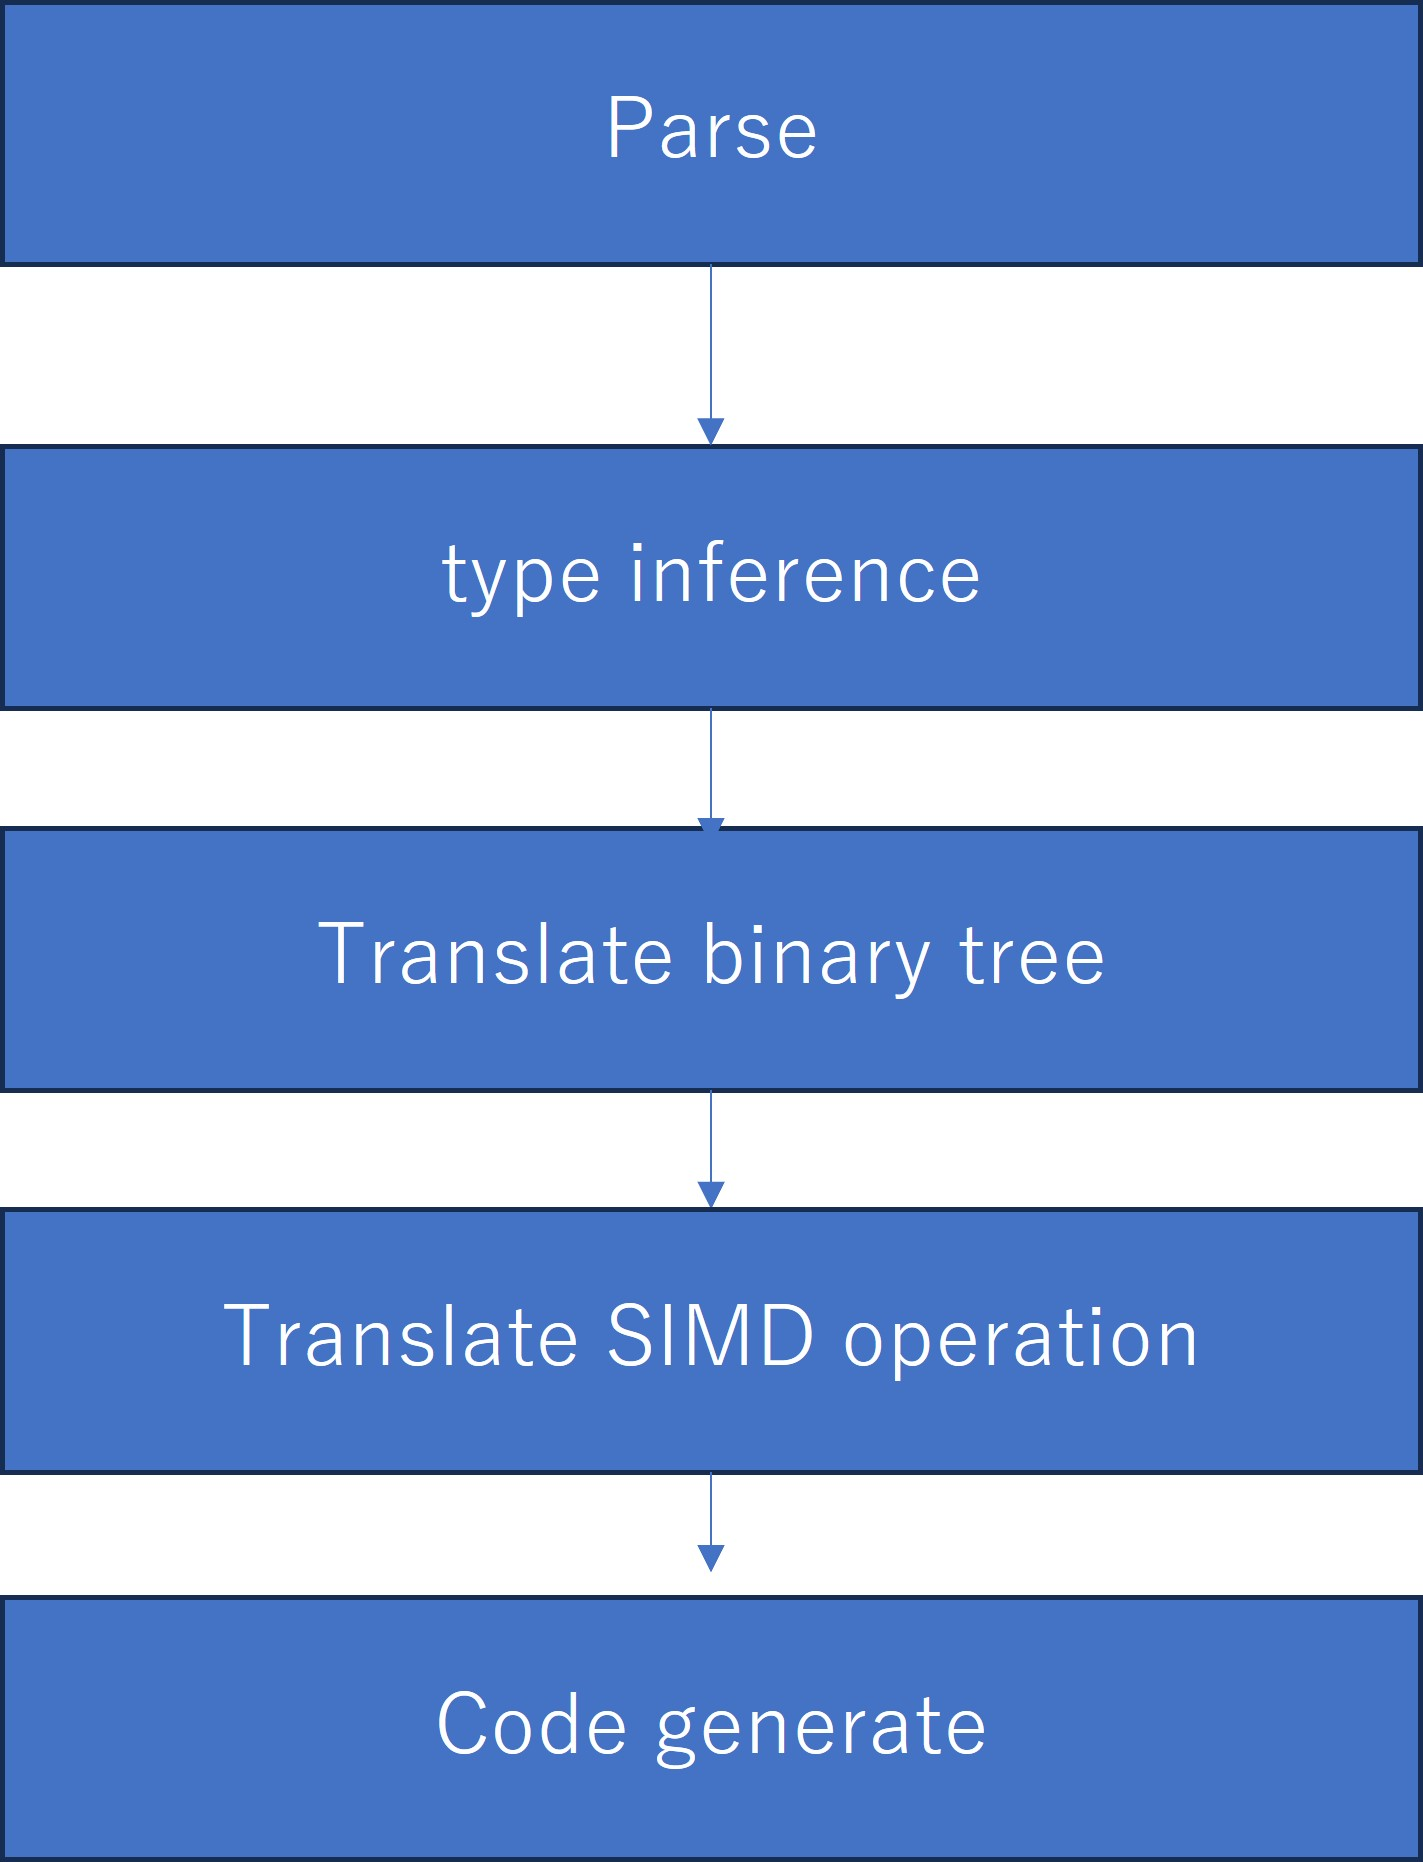
\includegraphics[width=\columnwidth]{../flowchartver4.jpg}
\caption{ここに画像のキャプションを入力}
\label{fig:image1}
\end{figure}

\end{document}